\chapter{Einf�hrung in die Programmierung eines EEXCESS--Clients}
\section{Grundlegendes}
Die Kommunikation eines Clients mit dem EEXCESS--Server basiert auf
dem Austausch von JSON--Objekten. Im Rahmen des
\SECH--Browser--Projektes werden nur die Dienste des
Privacy--Proxy--Service\footnote{Im Folgenden mit PP--Service
  abgek�rzt.}  in Anspruch genommen. Die daf�r ben�tigten
JSON--Objekte sind in der Online--Dokumentation des EEXCESS--Projektes
auf Github beschrieben.

\section{Informationsanfrage}
Informationsanfragen an den PP--Server geschehen in der Regel in zwei
Schritten.

\begin{figure}[ht]
    \centering
    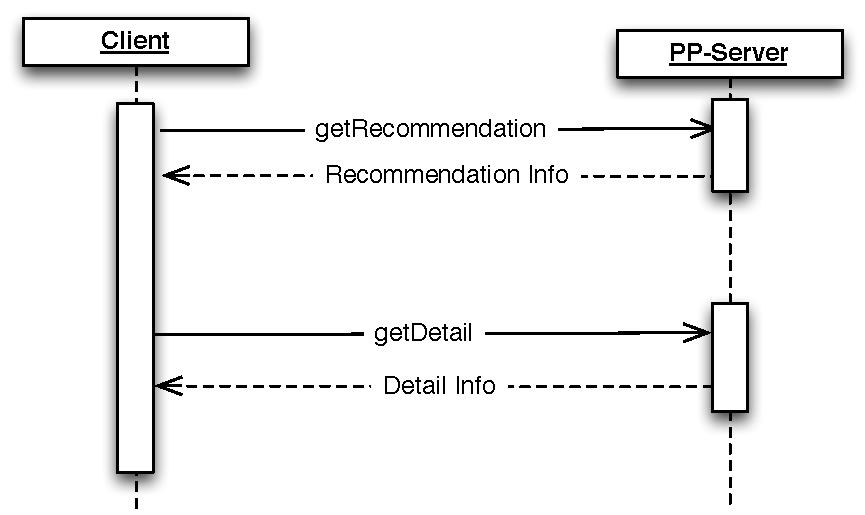
\includegraphics[width=0.75\textwidth]{clientServerComm}
    \caption{Beispiel f�r Informationsanfrage an den EEXCESS PP--Service}
    \label{fig:clientServerEEXCESS}
\end{figure}

Im ersten Schritt wird eine durch Suchparameter beschriebene
\Verb|/recommend|--Anfrage an der Server gestellt. Die Antwort darauf
besteht aus einem JSON--Objekt. Es enth�lt, neben den eigentlichen
Ergebnissen der Suchanfrage, auch eine eineindeutige Id zur sp�teren
Referenzierung der Anfrage. Die zur�ckgelieferten Ergebnisse bestehen
ihrerseits wieder aus verschiedenen Elementen, unter anderem einem
Titel der das Element n�her beschreibt, einer URI die angibt wo das
Objekt gespeichert ist und einer eineindeutigen Id zur Referenzierung
des Objekts. Diese Informationen w�rden bereits ausreichen, um die einzelnen
Ergebnisse der Suchanfrage aus dem Netz zu laden. Da der Benutzer aber
selber entscheiden soll, ob die angezeigten Zusatzinformationen f�r
ihn interessant sein k�nnten, muss er vor der Darstellung eine Auswahl
treffen k�nnen. Dies ist an Hand des Titels in der Regel nur schwer
m�glich!

In einem zweiten, optionalen Schritt kann daher f�r jedes Ergebnis
einer \Verb|/recommend|--Anfrage eine detaillierte Kurzbeschreibung
vom PP--Server abgerufen werden. Der daf�r vorgesehene
\Verb|/getDetails|--Befehl �bergibt die Id der Suchanfrage und die
\Verb|documentBadge|--Informationen des urspr�nglichen Ergebnisses an
den PP--Server und bekommt, falls bei der Datenquelle hinterlegt, eine
Kurzbeschreibung des Ergebnisses. An Hand dieser Kurzbeschreibung kann
der Anwender dann entscheiden, ob das eigentliche Informations--Objekt
�ber die zugeordnete URI geladen werden soll oder nicht.

\subsection{\texttt{/recommend}--Anfrage im \SECH--Browser Projekt}
Ein minimales JSON--Objekt f�r eine \Verb|/recommend|
Anfrage an den PP--Server besteht aus 3~Teilen:
\begin{enumerate}
     \item Den \Verb|origin| Informationen, die den Client n�her beschreiben.
     \item Dem \Verb|loggingLevel|, der angibt ob der PP--Server die
    Anfragen aufzeichnen darf oder nicht.
    \item Den \Verb|contextKeywords|, die die eigentlichen
   Suchbegriffe beinhalten.
\end{enumerate}

�ber weitere Parameter k�nnen die \Verb|/recommend|--Anfrage noch
genauer definiert werden. Im \SECH--Browser werden folgende
Parameter verwendet:
\begin{enumerate}
     \item \Verb|numResults|, um die Anzahl der vom PP-Server
    zur�ckgegebenen Resultate begrenzen zu k�nnen.
     \item Das \Verb|isMainTopic| Attribut der \Verb|contextKeywords|
    Eintr�ge, um bei mehreren Suchparametern eine Priorisierung
    durchf�hren zu k�nnen.
     \item \Verb|interests|, um die Anfragen genauer an die Vorlieben
    des Benutzers anpassen zu k�nnen.
     \item \Verb|languages|, um bevorzugt \SECH--Annotations in der
    Muttersprache des Benutzers zu verwenden.
     \item \Verb|timeRange|, um die \SECH--Annotations zeitlich
    eingrenzen zu k�nnen.
\end{enumerate}

Falls vom PP--Server unterst�tzt, sollen auch folgende Parameter zur
n�heren Beschreibung der Suchanfrage verwendet werden:
\begin{itemize}
     \item \Verb|ageRange|
     \item \Verb|gender|
     \item \Verb|address|
\end{itemize}